\documentclass[11pt, a4paper, twoside]{article}

\usepackage{a4wide}
\usepackage[USenglish, ngerman]{babel}
\usepackage[latin1]{inputenc}
\usepackage[T1]{fontenc}
\usepackage{makeidx}
\usepackage{url}
\usepackage{doc}
\usepackage{graphicx}
\usepackage{lmodern} 
\usepackage{amsmath}
\usepackage{amssymb}
\usepackage{pdfpages}
\usepackage{hyperref}
\usepackage{fancyheadings}
\usepackage{amsfonts}
\usepackage{amsthm}
\usepackage{color}
\usepackage{stmaryrd}
\usepackage{nomencl}
\usepackage[normalem]{ulem} 
\newcommand{\markup}[1]{\uline{#1}}
% Befehl umbenennen in abk
\let\abk\nomenclature
% Deutsche "uberschrift
\renewcommand{\nomname}{Abk\"urzungsverzeichnis}
% Punkte zw. Abk"urzung und Erklärung
\setlength{\nomlabelwidth}{.20\hsize}
\renewcommand{\nomlabel}[1]{#1 \dotfill}
% Zeilenabstände verkleinern
\setlength{\nomitemsep}{-\parsep}
\makenomenclature
\newcommand{\rf}{\color{red}}
\newcommand{\wf}{\color{white}}
\newcommand{\tf}{\color{black}}

%Kopf- und Fu"szeile
\usepackage{fancyhdr}
\pagestyle{fancy}
\fancyhf{}

%Kopfzeile links bzw. innen
\fancyhead[L]{\scshape\leftmark}
%Linie oben
\renewcommand{\headrulewidth}{0.5pt}

%Fu"szeile links bzw. innen
\fancyfoot[C]{\thepage}
%Linie unten
\renewcommand{\footrulewidth}{0.5pt}
\emergencystretch=3em

% Umgebungen f"ur Sätze usw.
\newtheorem*{bemerkung*}{Bemerkung}
\newtheorem*{defi}{Definition}
\newtheorem*{defi*}{Definition}
\newtheorem*{bezeichnungen}{Bezeichnungen}
\newtheorem*{fakt}{Fakt}
\newtheorem*{beispiel}{Beispiel}
\newtheorem*{bsp}{Beispiel}
\newtheorem*{beispiel*}{Beispiel}
\newtheorem*{satz}{Satz}
\newtheorem*{satz*}{Satz}
\newtheorem*{lem}{Lemma}
\newtheorem*{protokoll*}{Protokoll}
\newtheorem*{idee}{Idee}

%definition of new commands
\newcommand{\DGEF}{\text{\textbf{DGEF}}}

\numberwithin{equation}{section}
\begin{document}


\begin{titlepage}
\pagenumbering{roman}
\begin{center}

\includegraphics[height=4cm]{hhulogo.jpg}\\
\vspace{1em}
\textbf{
\Large Heinrich-Heine-Universit"at D"usseldorf\\
\smallskip
\Large Institut f"ur Informatik\\
\smallskip}

\vspace{3em}
{\Huge Bachelorarbeit}

\vspace{4em} {\Huge Der Einfluss von nicht ehrlichen \\ \vspace{1em} Strategien auf den DGEF}
\end{center}

\vfill

\begin{center}
{\large
\begin{tabular}[l]{ll}
Name: & Alina Elterman\\
Matrikelnummer: & 1810231\\
Betreuer: & Prof. Dr. J"org Rothe\\
Abgabedatum: & 01.02.2011
\end{tabular}
}
\end{center}
\end{titlepage}
\newpage
\thispagestyle{empty}
\tableofcontents
\newpage
\thispagestyle{empty}
\printnomenclature
\newpage
\thispagestyle{empty}
\phantomsection
\listoffigures
\newpage
\pagenumbering{arabic}
\setcounter{page}{1}
\section{Einleitung}
Cake-Cutting: Was ist das eigentlich?\\
Viele Eltern qu"alen sich, wenn es darum geht, auf einem Geburtstag, gerecht den Kuchen unter den Kindern aufzuteilen. Man m"ochte alle Kinder gl"ucklich machen und jedem ein solches St"uck geben, dass es damit zufrieden ist und kein anderes haben m"ochte. Also wie l"asst sich das Problem l"osen?\\
Viele interdisziplin"are Wissenschaften, beispielweise in den Natur-, Geistes- und Wirtschaftswissenschaften versuchen eine L"osung auf die eben genannte Problematik zu geben.\footnote{Die genauen Schwerpunkte dieser Gebiete werden in Kapitel 2 aufgelistet.}\\
Doch nicht jeder Kuchen ist gleich. So kann die Form variieren und auch die M"oglichkeiten diesen zu teilen k"onnen sich unterscheiden.\footnote{Es wird eine Einf"uhrung in die M"oglichkeiten und Arten der Teilungen in Kapitel 3 gemacht.}\\
Einen Kuchen zwischen zwei Kindern aufzuteilen, ist der leichteste Fall. Dieses Verfahren nennt sich Cut \& Choose (-Protokoll) und wird im nachfolgenden erkl"art. Bei drei Kindern birgt das mathematische Verfahren Selfridge-Conway (-Protokoll) eine L"osung.\footnote{Eine "Ubersicht der bekannten Protokolle wird in Kapitel 4 gegeben.} F"ur vier Kinder existiert eine Ausnahmel"osung, f"ur f"unf konnte bis jetzt kein allgemeing"ultiges Protokoll aufgestellt werden.\\
Genau an dieser Stelle liegt eine der Problematiken dieser Arbeit. Wie l"asst sich dieser Zwiespalt l"osen?\\
Seit den 40er Jahren befassen sich verschiedene Wissenschaftler und Theoretiker mit dem Teilgebiet Cake-Cutting. Immer wieder ergibt sich die Frage nach dem gerechten Teilen. Als Begr"under und Problemsteller dieser Theorie gilt Hugo Dionizy Steinhaus in \cite{7} und \cite{17}. Ein weiteres Ph"anomen das sich beim Cake-Cutting bemerkbar macht, ist der Aspekt des Neides. Der Wirtschaftswissenschaftler Duncan Foley f"uhrte den Begriff der ''Neidfreiheit'' in \cite{8} ein. George Gamow und Marvin Stern haben sich am Beispiel des Weinteilungsproblems mit diesem Thema befasst und erweiterten die Fragestellung auf eine beliebige Anzahl von Personen in \cite{18}.\\
In den letzten Jahrzenten wurde viel in diesem Gebiet geforscht und das Interesse von den Computerwissenschaften geweckt. Hier liegt die Analyse der Komplexit"at solcher Aufteilungen im Vordergrund. Die Arbeit von Ariel Procaccia \cite{9} legte einen Meilenstein in der Komlexit"atsanalyse von neidfreien Cake-Cutting-Protokollen.\footnote{Das Verfahren wird in Kapitel 6 beschrieben und anhand eines Beispiels demonstriert.}\\
Im Folgenden, befasst sich diese Arbeit mit der Fragestellung von Steinhaus und den erzielten Fortschritten von ihm und seinen Kollegen. Dabei wird versucht neue Ans"atze und Perspektiven zu er"offnen.
%Kapitel 7 besteht aus der Zusammenfassung mit dem Ausblick auf neue %Forschungen und einem Simulationsmodell um auf eine neue Art die %Neidfreiheit in Protokollen zu pr"ufen und vergleichen zu k"onnen.
\newpage
\section{Grundlagen}
F"ur die gerechte Aufteilung m"ussen zun"achst alle M"oglichkeiten definiert werden welches Objekt, mit welchem Ziel, auf welche Art und Weise und zwischen welchen Subjekten aufgeteilt werden kann. Die Definitionen und grundlegende Annahmen wurden aus den B"uchern \cite{26} und \cite{27} entnommen.
\subsection{Grundbegriffe des Cake-Cutting}
Sei $P_n$=$\{p_1,...,p_n\}$ die Menge von $n$ \underline{Spieler}, die gemeinsam ein Objekt aufteilen m"ochten. Es wird angenommen, dass jeder von ihnen m"oglichst viel von diesem Objekt haben m"ochte.\footnote{Im Gegensatz dazu werden in der Literatur auch F"alle "uber Aufteilung von unerw"unschten Objekten (Chore Division) behandelt, z.B. zus"atzliche Arbeit, wo alle daran interessiert sind m"oglichst, wenig zu erhalten.}\\
%Au"serdem sind die Spieler nur an ihrem eigenen Wohl interessiert, d.h., %die Verschlechterung oder Verbesserung der Situationen von ihren %Mitspielern hat keinen direkten Einfluss auf ihr Wohlbefinden.\\
\newline
\textbf{Der Kuchen}\\
\newline
Im folgenden geht es nur um die Aufteilung von einem einzigen, heterogenen, beliebig teilbaren Gut.\footnote{Es existieren auch Forschungen "uber die Aufteilung von mehreren G"utern (z.B. \cite{1}), die  hier aber au"ser Acht gelassen wird.} Zur Veranschaulichung wird ein \underline{rechteckiger Kuchen} (Stollen) verwendet. \footnote{Es gibt mehrere Studien von einer Torte (runder Kuchen) nachzulesen in \cite{31}).}
\begin{figure}[h!]
\center
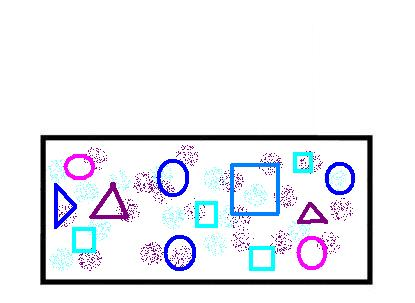
\includegraphics[height=4cm]{kuch.jpg}
\caption[Beispiel f"ur einen Kuchen]{Ein rechteckiger Kuchen mit unterschiedlichen Merkmalen vgl.\cite{25}. Die einzelnen Fragmente sind unterschiedlich wertvoll f"ur die Spieler.}
\end{figure} Die Division wird durch eine Reihe von parallen Schnitten durchgef"uhrt.\footnote{Es gibt ebenfalls Aufteilungen mit parallelen und rechtwinkligen Schnitten (z.B. Protokoll von Webb).} Der Kuchen $X$ wird dabei durch das Intervall $I=[0,1]\subseteq \mathbb{R}$ repr"asentiert. Jedes Teilintervall $I'\subseteq I$, oder eine Vereinigung von solchen, wird als \underline{St"uck} bezeichnet. Diese St"ucke sind immer disjunkt. Das St"uck des Kuchens, welches der Spieler $p_i$ bekommt, wird \underline{Portion} genannt und als $X_i$ bezeichnet. Jedes St"uck hat eine objektive L"ange, welche der Summe der Differenzen seiner Grenzen entspricht und eine subjektive Bewertung, die folgend entsteht:\\
\newline
\textbf{Die Bewertung} \\
\newline
Jeder Spieler $p_i \in P_N$ besitzt eine Bewertungsfunktion (Bewertung) $v_i:\{X'|X'\subseteq X\}\mapsto [0,1]$ des Kuchens $X$. Sie erf"ullt folgende Eigenschaften\footnote{vgl. zus"atzlich \cite{24}}:
\begin{enumerate}
\item Nicht-Negativit"at\footnote{manchmal auch Positivit"at: $v_i(C)> 0$ f"ur alle $C\subseteq [0,1], C \neq \emptyset.$}: $v_i(C)\geq 0$ f"ur alle $C\subseteq [0,1].$
\item Normalisierung: $v_i(\emptyset)=0$ und $v_i([0,1])=1.$
\item Monotonit"at: Wenn $C' \subseteq C$, dann $v_i(C') \leq v_i(C).$
\item Additivit"at: $v_i(C \cup C')=v_i(C)+v_i(C')$ f"ur disjunkte $C,C'\subseteq [0,1].$
\item Teilbarkeit\footnote{daraus folgt auch die Inhaltslosigkeit von Punkten:  $v_i([x,x])=0$ f"ur alle $x\in [0,1].$}: F"ur alle $C\subseteq [0,1]$ und alle $\alpha \in \mathbb{R}$, $0\leq \alpha \leq 1$, existiert ein $B\subseteq C$, so dass  $v_i(B)=\alpha \cdot v_i(C).$
\item  $v_i$ ist kontinuierlich: Falls $0<x<y\leq 1$ mit $v_i([0,x])=\alpha$ und $v_i([0,y])=\beta$, dann gilt f"ur jedes $\gamma \in [\alpha,\beta]$ existiert ein $z \in [x,y]$ so dass $v_i([0,z])=\gamma.$
\end{enumerate}
Bei den Beispielen wird die folgende Darstellung f"ur den Kuchen und deren Bewertung genutzt:\\
\newline
Die \textbf{Boxendarstellung}:
\begin{figure}[h!]
\center
 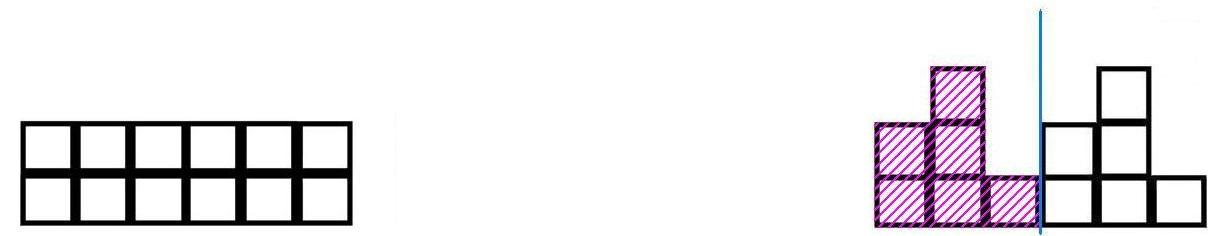
\includegraphics[height=3cm]{cc1svv.jpg}
\caption[Beispiel f"ur die Boxendarstellung eines Kuchens]{Eigenschaften: Ein solches Diagramm muss separat f"ur jeden Spieler erstellt werden. Die Anzahl der K"astchen ist bei allen Spielern gleich und diese repr"asentieren immer den gleichen Wert des Kuchens. Ab hier wird der Wert des Kuchens pro K"astchen genau $1/12$ und er wird linear auf der Fl"ache des K"astchens verteilt, z.B: 1/2 K"astchen = 1/24 der Kuchens. Die L"ange des Kuchens ist bei allen Spielern einheitlich sechs K"astchen. Diese Einschr"ankungen der Eigenschaften werden gemacht um die Beispiele verst"andlicher und einfacher zu machen. Der objektive Wert eines Kuchens sieht wie die linke Abbildung aus. Es werden die zw"olf K"astchen nach der jeweiligen Bewertung des Spieler verteilt, wie z.B. in der rechten Abbildung. Die straffierte Fl"ache ist das St"uck, welches der jeweilige Spieler erh"alt und dessen Summe ist der Wert seines St"uckes. Die parallelen Schnitte werden wie abgebildet eingezeichnet.}
\end{figure}
\newline
\textbf{Die unterschiedlichen Arten von Gerechtigkeit}\\
\newline
Wie oben bereits definiert wurde, besitzt jeder Spieler eine Bewertungsfunktion. Diese Funktion ist geheim und subjektiv (ein Spieler kennt nur seine Bewertungen, und nur seine Bewertungen haben Einfluss auf sein Wohlbefinden). Nach einer Aufteilung wird die G"ute dieser gemessen. Daf"ur werden Ma"sst"abe ben"otigt. Der Wichtigste ist die Gerechtigkeit. Aber was bedeutet "uberhaupt gerecht? Dies ist eine philosophische oder psychologische Frage und kann nicht so einfach und f"ur das gegebene Ziel zufriedenstellend beantwortet werden. Also werden Kriterien ben"otigt um die Aufteilungen untereinander vergleichen und bewerten zu k"onnen. Alle Kriterien sind als subjektive Einsch"atzungen von den Spielern und nicht alss objektive Ma"sst"abe zu verstehen. 
\begin{defi}{\textbf{(Proportionalit"at oder einfache Gerechtigkeit)}}
\newline Eine Aufteilung ist \underline{proportional (einfach gerecht)}, falls  $v_i(X_i) \geq 1/n$ f"ur jeden Spieler $p_i \in P_N$ gilt. 
\end{defi} 
\begin{defi}{\textbf{(Neidfreiheit)}}
\newline Eine Aufteilung ist \underline{neidfrei}, falls $v_i(X_i) \geq v_i(X_j)$ f"ur jedes Paar von Spielern $p_i, p_j \in P_N$. 
\end{defi}
\begin{defi}{\textbf{(Starke Neidfreiheit)}}
\newline  Eine Aufteilung ist \underline{stark-neidfrei} falls $v_i(X_i) > v_i(X_j)$ f"ur jedes Paar von Spielern $p_i, p_j \in P_N, i \neq j$.  
\end{defi} 
\begin{defi}{\textbf{(Super Neidfreiheit)}}
\newline Eine Aufteilung ist \underline{super-neidfrei}, falls $v_i(X_j) \leq 1/n$  f"ur jedes Paar von Spielern $p_i, p_j \in P_N, i \neq j$. 
\end{defi} 
\begin{defi}{\textbf{(Starke Super Neidfreiheit)}}
\newline Eine Aufteilung ist \underline{stark-super-neidfrei}, falls $v_i(X_j) < 1/n$  f"ur jedes Paar von Spielern $p_i, p_j \in P_N, i \neq j$. 
\end{defi} 
Das Problem ist, dass f"ur die st"arkeren Einschr"ankungen nicht immer Aufteilungen existieren, z.B. wenn alle Spieler die gleiche Bewertungsfunktion auf den Kuchen besitzen. 
\begin{defi}{\textbf{(Exaktheit)\footnote{In der Literatur wird an Stelle von Exaktheit oft der Begriff der Gerechtigkeit verwendet, was in gewissem Sinne den gesamten Konzept der Begriffe widerspricht, da alle diese Kriterien einzeln als unterschiedliche Ma"sst"abe von gerecht befunden werden.}}}
\newline Eine Aufteilung ist \underline{exakt}, falls $v_i(X_i) = v_j(X_j)$ f"ur jedes Paar von Spielern $p_i, p_j \in P_N$.
\end{defi}
In wirtschaftlichen Texten werden Aufteilungen, die gleichzeitig exakt und neidfrei, sind oft als besonders gerecht empfunden. Dennoch hat die Exaktheit sogar in Kombination mit der Proportionalit"at keinen direkten Zusammenhang mit der Neidfreiheit, wie man sich am folgenden Beispiel leicht veranschaulichen kann.\\
\begin{bsp}Die Spieler Aleph, Beth und Gimel teilen einen Kuchen. Am Ende bekommt jeder Spieler genau $1/3$ des Kuchens (nach seinem Ma"s). Diese Aufteilung ist exakt und proportional. Doch Aleph ist der Meinung, dasgBeths St"uck genau die H"alfte des Kuchens ist und beneidet Beth. Damit ist die Aufteilung nicht neidfrei.\end{bsp}
\textbf{Zusammenh"ange der Gerechtigkeitskriterien:}
\begin{lem}
F"ur alle Aufteilungen gilt:
\begin{enumerate}
\item Falls eine Aufteilung neidfrei ist, so ist sie auch proportional.
\item F"ur zwei Spieler ist eine Aufteilung proportional genau dann, wenn sie neidfrei ist.
\end{enumerate}
\end{lem}
\begin{proof}
\begin{enumerate}
\item Beweis durch Widerspruch:\\ Sei $A$ eine Aufteilung die neidfrei, aber nicht proportional ist. Da die Aufteilung $A$ neidfrei ist, gilt $v_i(X_i) \geq v_i(X_j)$ f"ur jedes Paar von Spielern $p_i, p_j \in P_N$ und somit hat jeder Spieler mind. soviel wie jeder andere. Daraus folgt, dass jeder Spieler mindestens genauso viel wie $(n-1)$ andere hat und somit mindestens $1/n$. Damit ist die Aufteilung $A$ proportional. $\lightning$\\Somit sind alle neidfreien Aufteilungen proportional.
\item ''$\Rightarrow$'' F"ur zwei Spieler ist eine Aufteilung proportional, wenn er mind. die H"alfte des Kuchens bekommt, damit kann der andere Spieler h"ochstens die H"alfte bekommen und wird nicht beneidet.\\ ''$\Leftarrow$'' Die R"uckrichtung folgt aus Zusammenhang 1.\\
\end{enumerate}
\end{proof}
\begin{defi}{\textbf{(Effizienz)}}
\newline Eine Aufteilung ist \underline{effizient (Pareto optimal)}, falls keine andere Aufteilung existiert, die einem Spieler ein von ihm besser bewertetes St"uck einbringt, ohne die Situation eines anderen Spielers zu verschlechtern. 
\end{defi}
\subsection{Grundbegriffe der Spieltheorie}
\begin{defi}{\textbf{(Risikoaversion)\footnote{In den letzten Jahren wurde dieser Aspekt konzentrierter untersucht vgl. \cite{23}. Es kann als ein einzelnes Kriterium formuliert werden.}}}
\newline Eine Aufteilung (Prozedur) ist \underline{ehrlich}, falls es keine Bewertungen gibt, bei der Spieler am Ende durch Unaufrichtigkeit ein wertvolleres St"uck bekommen h"atten. \footnote{''We say that a cake cutting procedure is truthful iff there are no valuations where a player will do better by lying.'' aus \cite{41}.}
\end{defi}
\begin{defi}{\textbf{(Ehrlichkeit)\footnote{In den letzten Jahren wurde dieser Aspekt konzentrierter untersucht vgl. \cite{23}. Es kann als ein einzelnes Kriterium formuliert werden.}}}
\newline Eine Aufteilung (Prozedur) ist \underline{ehrlich}, falls es keine Bewertungen gibt, bei der Spieler am Ende durch Unaufrichtigkeit ein wertvolleres St"uck bekommen h"atten. \footnote{''We say that a cake cutting procedure is truthful iff there are no valuations where a player will do better by lying.'' aus \cite{41}.}
\end{defi}
Es besteht nur Interesse an Aufteilungen, wo die Ehrlichkeit die beste Strategie f"ur alle Spieler ist und somit allein durch den Algorithmus erzwungen wird. Oft wird dies erreicht, indem der Spieler durch Unaufrichtigkeit Gefahr l"auft die Garantie auf seinen gerechten Anteil zu verlieren.\\
\subsection{Grundbegriffe der Komplexit"atsanalyse von Protokollen}
\textbf{Komplexit"atsklassen\footnote{aus \cite{19}}}\\
\newline
Um Algorithmen anhand ihrer Laufzeiten besser zuordnen und vergleichen zu k"onnen wurden die zwei nachfolgenden Funktionenklassen eingef"uhrt.
$$\mathcal{O}(g)= \{f :\mathbb{N} \mapsto \mathbb{N} | (\exists c >0)(\exists n_0 \in \mathbb{N}) (\forall n \geq n_0) [f(n) \leq c \cdot g(n)]\}$$
 Die Funktion $f \in \mathcal{O}(g)$ w"achst asymptotisch nicht schneller als $g$. Es d"urfen Konstanten und endlich viele Ausnahmen vernachl"assigt werden. Die Funktion $g$ wird als \underline{obere Schranke} bezeichnet. In dieser Funktionsklasse liegt immer der \underline{ung"unstigste Fall}. Dies ist eine g"ultige Eingabe, f"ur dessen L"osung der Algorithmus die l"angste Zeit ben"otigt. \\
$$\Omega(g)= \{f :\mathbb{N} \mapsto \mathbb{N} | (\exists c >0)(\exists n_0 \in \mathbb{N}) (\forall n \geq n_0) [f(n) \geq c \cdot g(n)]\}$$
 Die Funktion $g$ w"achst asymptotisch nicht schneller als jedes $f \in \Omega(g)$. Die Funktion $g$ wird als \underline{untere Schranke} bezeichnet. In dieser Funktionsklasse liegt immer der \underline{beste Fall}. "Ublicherweise ist diese Zeitangabe kleiner als das tats"achliche Resultat, aber man kann beweisen, dass ohne diesen Zeitaufwand das Problem nicht l"osbar ist.\\
\newline
\textbf{Klassen von Protokollen}\\
\newline
Intuitive Beschreibung: \underline{Algorithmus}
\newline In der Mathematik, Informatik und verwandten Gebieten, ist ein Algorithmus eine effektive Methode zur Probleml"osung, ausgedr"uckt durch eine endliche Folge von Anweisungen.
\begin{defi}{\textbf{(Protokoll (Cake-Cutting-Protokoll)\footnote{Vgl. mit Definition aus \cite{3}, \cite{35} und \cite{24} oder \cite{34}\abk{CC}{\markup{C}ake-\markup{C}utting}.}
)}}
\newline Ein \underline{Protokoll (Cake-Cutting-Protokoll)} ist ein Algorithmus mit mehreren Spielern und folgenden Eigenschaften:
\begin{itemize}
\item{Es besteht aus Regeln und Strategien.\\ \underline{Regeln} sind Anweisungen, die gefordert werden ohne die Bewertungen der Spieler zu kennen (deren Befolgung kann kontrolliert werden).\\ \underline{Strategien} sind Empfehlungen, welchen der Spieler folgen kann um garantiert seinen gerechten Anteil zu bekommen.
}
\item{Sofern ein Spieler sich nicht an die Strategie des Protokolls h"alt, verliert er seinen Anspruch nach einer endlichen Anzahl von Schritten ein St"uck des Kuchens zu bekommen, welches dem geforderten Gerechtigkeitskriterium entspricht. Sein Vorgehen hat aber keine Auswirkungen auf die Anteile der anderen Spieler.}
\item Jeder Spieler muss zu jeder Zeit in der Lage sein, v"ollig unabh"angig von den anderen Spielern den Kuchen zu teilen (einen Schnitt zu machen).
\item Das Protokoll besitzt keine Informationen "uber die Bewertungen der Spieler, ausser denen die angefragt wurden in dem jeweiligen oder in den vorherigen Schritten.
\end{itemize}
\begin{bsp}
Regel:\\ Spieler $p_1$ schneide ein St"uck ab.
Strategien:\\ Spieler $p_1$ halbiere das St"uck nach seinem M"a"s.
\end{bsp}
\end{defi}
\begin{defi}
Ein Cake-Cutting-Protokoll wird proportional, neidfrei, stark neidfrei etc. genannt, falls unabh"angig von den Bewertungsfunktionen der Spieler, jede Aufteilung entsprechend proportional, neidfrei etc., unter der Vorraussetzung, dass alle Spieler die vom Protokoll vorgegebenen Regeln und Strategien befolgen, ist.
\end{defi}
Eines der Ziele von Cake-Cutting ist solche Protokolle anzugeben.\begin{defi}{\textbf{(endlich (diskret)/kontinuierlich)}}
\newline Ein \underline{endliches (diskretes)} Protokoll liefert eine L"osung nach einer endlichen Anzahl von Entscheidungen (Bewertungen, Markierungen,$\ldots$), dagegen muss ein Spieler bei einem \underline{kontinuierlichen} Protokoll unendlich viele Entscheidungen treffen.
\end{defi}
\begin{defi}{\textbf{(endlich beschr"ankt/endlich unbeschr"ankt))}}
\newline Ein \underline{endlich beschr"anktes} Protokoll hat eine obere Grenze von Schritten, welche im ung"unstigsten Fall betrachtet wird. Die gesamte Anzahl von Entscheidungen h"angt, wenn "uberhaupt, dann nur von der Anzahl der beteiligten Personen ab. Ein \underline{endlich unbeschr"anktes} Protokoll hat hingegen eine nicht im Voraus absch"atzbare Anzahl.
\end{defi}
Die begehrtesten Protokolle sind endlich beschr"ankt, da sie am einfachsten in der Realit"at umsetzbar sind. Aber es gibt eine Art von kontinuierlichen Protokollen, an denen ebenfalls Interesse besteht.
\begin{defi}{\textbf{(Moving-Knife-Protokoll)}}
\newline Ein Schiedsrichter, welcher unparteisch gegen"uber den Spielern ist und unbeteiligt an der Verteilung der St"ucke, \underline{schwenkt ein Messer kontinuierlich} von links nach rechts und macht parallele Schnitte sofern ein Spieler ''Halt!'' ruft. Bei manchen MKP\abk{MKP}{\markup{M}oving-\markup{K}nife-\markup{P}rotokoll} wird der Schiedsrichter ausgelassen und nur ein Messer oder Schwert geschwungen.
\end{defi}
Bemerkung: In der Literatur (z.B.: \cite{36}) werden manchmal kontinuierliche Protokolle nicht als Protokolle bezeichnet sondern zu neuen Klassen zusammengefasst, die von der Anzahl der Messer abh"angen.\\
\newline
 Eine weitere wichtige Eigenschaft von Cake-Cutting ist, dass nur komplette Aufteilungen des Kuchens,also wo jedes St"uck einem Spieler zugeordnet wird, betrachtet werden.

\section{Der Grad der garantierten Neidfreiheit}
\begin{description}
 \item[Motivation] F"ur $n\geq4$ ist es offen, ob es ein neidfreies, endlich beschr"anktes CCP gibt!
 \item[$\Rightarrow$] Abschw"achen des Ideals der Neidfreiheit. 
\end{description}
\begin{defi}
 Sei eine Aufteilung des Kuchens $X=\bigcup\limits_{i=1}^n X_i$ f"ur die Menge $P=\{p_1,\dots,p_n\}$ der Spieler gegeben, wobei $v_i$
 das Ma"s von $p_i$ und $X_i$ die Portion von $p_i$ ist.
 \begin{itemize}
  \item Eine \underline{Neidrelation}(``envy relation'') $\Vdash$ ist eine Bin"arrelation auf $P(\Vdash, PxP):p_i$ beneidet 
        $p_j$ $(p_i\Vdash p_j)$, $1\leq i,j\leq n,$ $i\neq j$, falls $v_i(X_i)<v_i(X_j)$.
  \item Eine \underline{Neidfrei-Relation} (``envy-free relation'') $\nVdash$ ist eine Bin"arrelation auf $P:p_i$ beneidet nicht $p_j$ $(p_j
        \nVdash p_j)$ ,$1\leq i,j\leq n$ ,$i\neq j$, falls $v_i(X_i)\geq v_i(X_j)$.
 \end{itemize}
\end{defi}
\underline{Eigenschaften von $\Vdash$ und $\nVdash$:}
\begin{itemize}
 \item $\Vdash$ ist irreflexiv, denn $v_i(X_i)<v_i(X_i)$ gilt nie
 \item $\nVdash$ ist reflexiv, denn $v_i(X_i)\geq v_i(X_i)$ gilt immer\\Die triviale Beziehung $p_i \nVdash p_i$ z"ahlt in der Regel nicht
       mit.
 \item $\Vdash$ und $\nVdash$ sind nicht transitiv.\\
       Gilt z.B. $p_i\Vdash p_j$ und $p_j\Vdash p_k$, so kann man daraus nichts "uber $v_i(X_k)$ schlie"sen: $p_i\nVdash p_k$ ist m"oglich
\end{itemize}
$\Rightarrow$ Es gibt die folgenden M"oglichkeiten:
\begin{enumerate}
 \item Zwei-Wege-Neid: $p_i\Vdash p_j$ und $p_j\Vdash p_i$\\(Tausch der Portionen macht beide gl"ucklich.)
 \item Zwei-Wege-Neidfreiheit: $p_i\nVdash p_j$ und $p_j\nVdash p_i$\\(Alles ist gut.)
 \item Ein-Weg-Neid: $p_i\Vdash p_j$ und $p_j\nVdash p_i$\\
       Ein-Weg-Neidfreiheit: $p_j\Vdash p_i$ und $p_i\nVdash p_j$
\end{enumerate}
Fallerzwungene Neid- bzw. Neidfrei-Relationen: h"angen ab von einem Fall geeigneter Ma"se.\\
Garantierte Neid- bzw. Neidfrei-Relationen: gelten in jeden Fall (auch im worst case), also unabh"angig von den Ma"sen der Spieler.\\
Anzahl garantierter Neidfrei-Relationen $=\min\limits_{alle Faelle}$ Anzahl der fallerzwungenen Neidfrei-Relationen.
%\includepdf[pages=17,scale=0.8]{folien.pdf}
\begin{beispiel*}
 Aufteilung $X=X_F\cup X_G\cup X_H$ des Kuchens mit\\
 \begin{tabular}{c|ccc}
  & $X_F=$\begin{tabular}{ccc}&&$\Box$\\&$\Box$&$\Box$\\$\Box$&$\Box$&$\Box$\\1&2&3\end{tabular}
  & $X_G=$\begin{tabular}{ccc}$\Box$&$\Box$&$\Box$\\7&8&9\end{tabular}
  & $X_H=$\begin{tabular}{ccc}$\Box$&$\Box$&$\Box$\\$\Box$&$\Box$&$\Box$\\4&5&6\end{tabular}\\ \hline \\
  F & \textcolor{blue}{$\frac{6}{18}=\frac{1}{3}$} & $\frac{6}{18}=\frac{1}{3}$ & $\frac{6}{18}=\frac{1}{3}$\\ \\
  G & $\frac{9}{18}=\frac{1}{2}$ & \textcolor{blue}{$\frac{3}{18}=\frac{1}{6}$} & $\frac{6}{18}=\frac{1}{3}$\\ \\
  H & $\frac{5}{18}$ & $\frac{7}{18}$ & \textcolor{blue}{$\frac{6}{18}=\frac{1}{3}$}
 \end{tabular}\\
 $\Rightarrow$ nicht proportional wegen $v_G(X_g)=\frac{1}{6}<\frac{1}{3}$.\\
 Es gibt:
 \begin{itemize}
  \item[] Ein-Weg-Neid von $G$ zu $F$:\\$G\Vdash F$ wegen $v_G(X_G)=\frac{1}{6}<v_G(X_F)=\frac{1}{2}$
          \\ Gleichzeitig ist dies\\$F\nVdash G$ wegen $v_F(X_G)=\frac{1}{3}=v_F(X_F)$
  \item[] Ein-Weg-Neidfreiheit von $F$ zu $G$
  \item[] Zwei-Wege-Neidfreiheit zwischen $F$ und $H$\\ $F\nVdash H$, da $v_F(X_F)=\frac{1}{3}=v_F(X_H)$\\
          $H\nVdash F$, da $v_H(X_H=\frac{6}{18}>\frac{5}{18}=v_H(X_F)$
  \item[] Zwei-Wege-Neid zwischen $G$ und $H$\\$G\Vdash H$, da $v_g(X_G)=\frac{1}{6}<\frac{1}{3}=v_G(X_H)$\\
          $H\Vdash G$, da $v_H(X_H)=\frac{1}{3}<\frac{7}{18}=v_H(X_G)$
 \end{itemize}
 %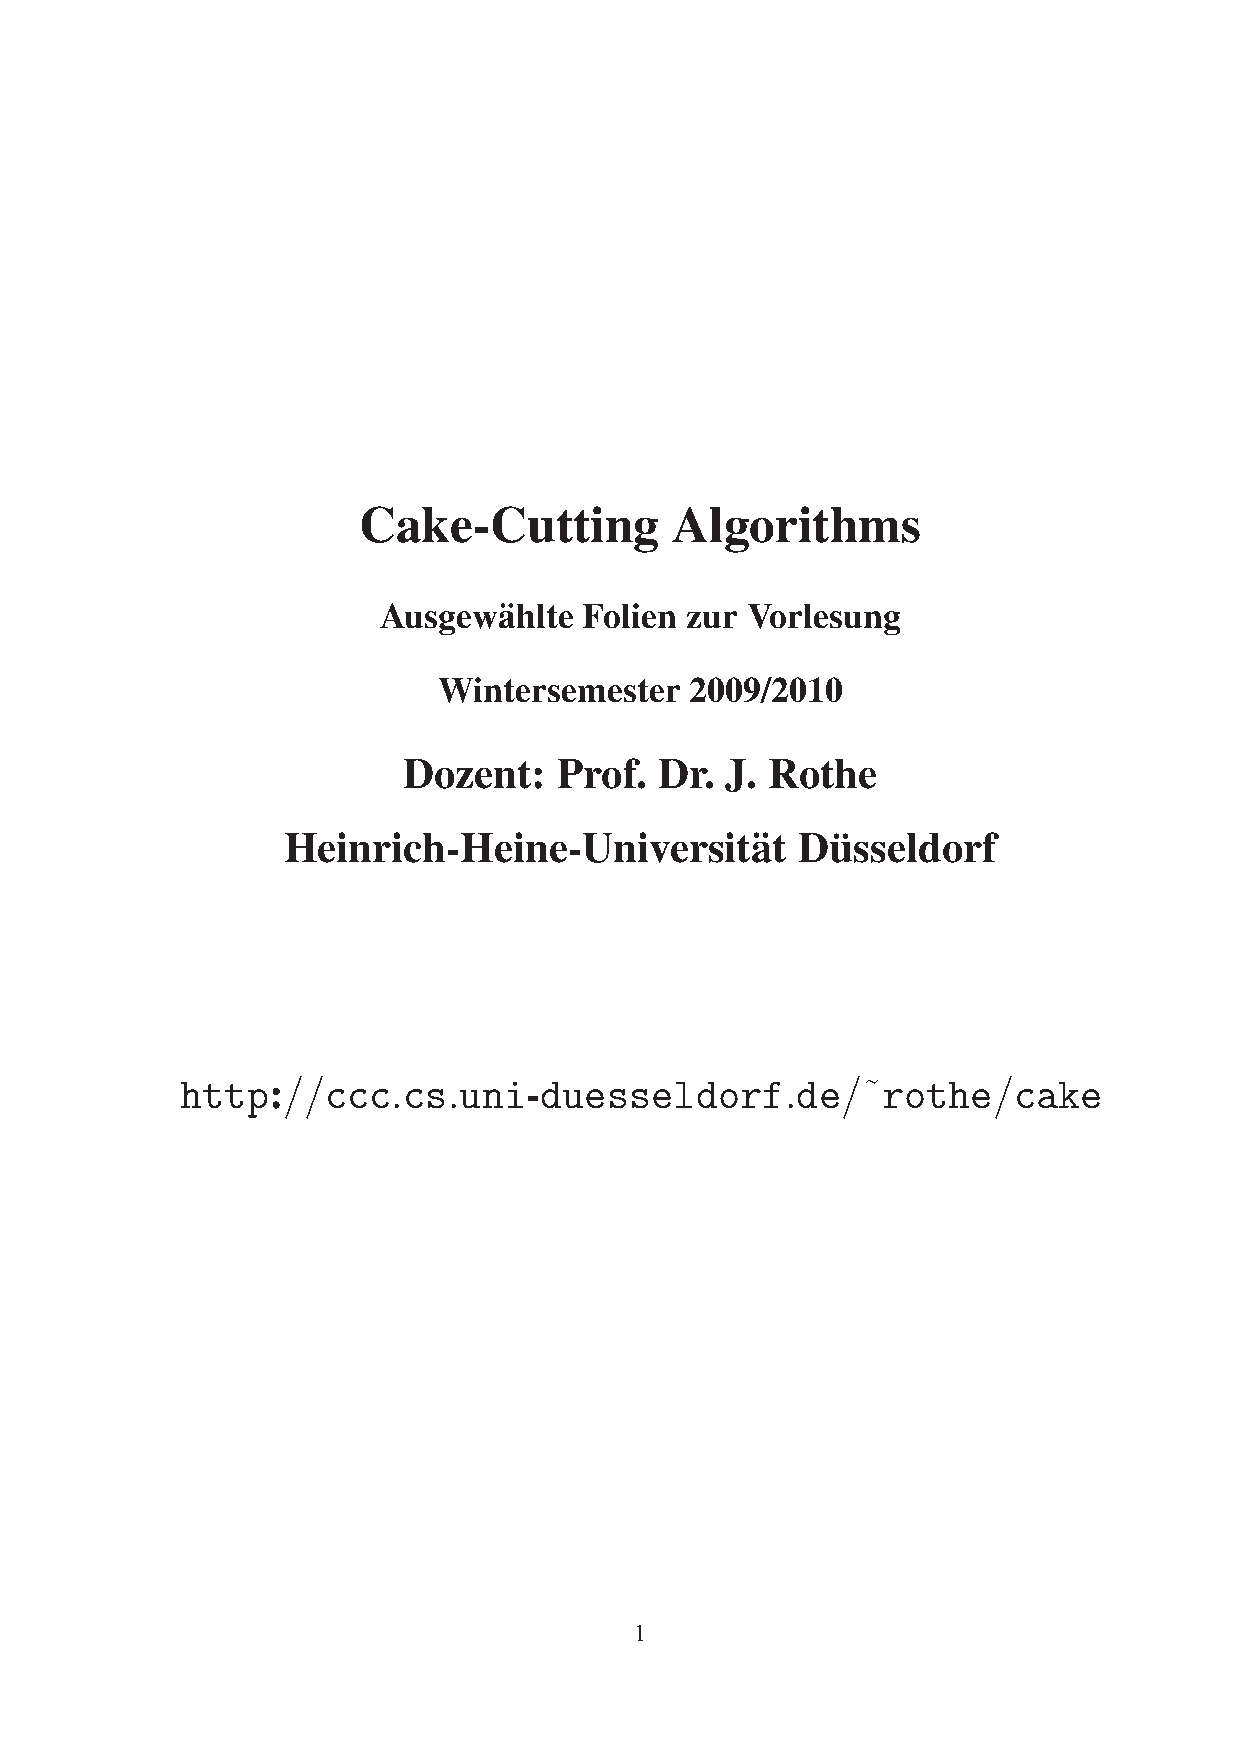
\includepdf[pages=K"astchenfolieBis9,scale=0.8]{folien.pdf}
\end{beispiel*}
$\DGEF =$ Anzahl der Neidfrei-Relationen im worst case
\begin{protokoll*}
 J"org erh"alt den Kuchen.\\
 $\DGEF: n-1+(n-1)(n-2)=n-1-n^2-3n+2=n^2-2n-1$
\end{protokoll*}
\begin{satz*}
 \begin{enumerate}
  \item Jedes neidfreie CCP f"ur $n\geq1$ Spieler hat einen $\DGEF$ von $n(n-1)$.
  \item Sei $d(n)$ der $\DGEF$ eines proportionalen CCPs mit $n\geq2$ Spielern. Dann gilt: $n\leq d(n)\leq n(n-1)$.
 \end{enumerate}
\end{satz*}
\begin{proof}
 \begin{enumerate}
  \item Da wir $p_i\nVdash p_i$ f"ur alle $i$, $1\leq i\leq n$, au"ser 8 lassen, hat jeder der $n$ Spieler zu jedem anderen Spieler eine
        Neidfreie-Relation, insgesamt also $n(n-1)$.
  \item \begin{description}
         \item[$n=2$] Offenbar gilt: $d(2)=2$, denn da das CCP proportional ist, gilt: $v_1(X_1)\geq\frac{1}{2}$ und $v_2(X_2)\geq\frac{1}{2}
                    \Rightarrow v_1(X_1)\geq v_1(X_2)$ und $v_2(X_2)\geq v_2(X_1)$
         \item[$n\geq3$] Da $p_i\nVdash p_i$ f"ur alle $i$ ignoriert wird, gilt $d(n)\leq n(n-1)$.
                         \begin{itemize}
                          \item[] In einer proportionalen Aufteilung gilt:\\$v_i(X_i)\geq\frac{1}{n}$ f"ur $1\leq i\leq n$.\\
                          \item[$\Rightarrow$] Keiner der $n$ Spieler kann gleichzeitig alle anderen Spieler bendeidenl, denn:\\
                                               Angenommen, das w"are nicht so. Konkret: $p_1\nVdash p_2$
                          \item[$\Rightarrow$]$v_1(X_2)>v_1(X_1)\geq\frac{1}{n}$
                          \item[$\Rightarrow$]$v_1((X-X_1)-X_2)<\frac{n-2}{n}$
                          \item[$\Rightarrow$]$(X-X_1)-X_2$ kann nicht so in $n-2$ Portionen aufgeteilt werden, dass $v_i(X_j)\geq\frac{1}{n}$
                                              f"ur alle $j,3\leq j\leq n$, gilt.
                          \item[$\Rightarrow$]es gibt ein $j,3\leq j\leq n$, so dass $v_i(X_j)<\frac{1}{n}$, gilt.
                          \item[$\Rightarrow$]$p_i\nVdash p_j$
                         \end{itemize}
                         Also hat jeder der $n$ Spieler mindestens eine garantierte Neidfrei-Relation zu einem anderen Spieler: $n\leq d(n)$  
        \end{description}
 \end{enumerate}
\end{proof}

\begin{lem}
 Verlangen die Regeln/Strategien eines proportionalen CCPs f"ur $n\geq2$ Spielern von keinem Spieler, die Portionen der anderen Spieler
 zu bewerten, dann ist der $\DGEF=n$.
\end{lem}
\begin{proof}
 \begin{description}
  \item[$n=2$] Proportionalit"at $\Rightarrow$ Neidfreiheit\\best case $=$ worst case\\und wie vorher: $\DGEF=2=n$
  \item[$n\geq3$] Betrachte das folgende Szenario: F"ur eine gegebene Aufteilung $X=\bigcup\limits_{i=1}^nX_i$, die proportional ist, aber sonst
                  keinerlei Einschr"ankungen unterliegt, setzen wir die Ma"se der Spieler so: \\F"ur jedes $i, 1\leq i\leq n$, bewertet $p_i$:
                  \begin{itemize}
                   \item die eigene Portion $X_i$ mit $v_i(X_i)=\frac{1}{n}=\frac{n}{n^2}\Rightarrow$ proportional!
                   \item die Portion $X_j$ eines Spielers $p_j, j\neq i: v_i(X_j)=\frac{2}{n}<\frac{1}{n}$
                   \item jede der $n-2$ "ubrigen Portionen $X_k$ der Spieler $p_k, |{i,j,k}|=3, v_i=(X_k)=\frac{n+1}{n^2}>\frac{1}{n}$
                  \end{itemize}
                  Insgesamt gilt dann f"ur jedes $i, 1\leq i\leq n$:
                  \begin{enumerate}
                   \item $v_i(X)=v_i(\bigcup\limits_{j=1}^nX_j)\stackrel{\text{Additivit"at}}{=}\sum\limits_{j=1}^nv_i(X_j)=
                         \frac{1}{n^2}(n+2+(n-2)(n+1))=\frac{1}{n^2}(n+2+n^2+n-2n-2)=1$
                   \item $p_i$ hat $n-2$ Neidrelationen und nur eine Neidfrei-Relation\\$\Rightarrow$ Insgesamt gibt es $n$ garantierte 
                         Neidfrei-Relationen, eine f"ur jeden Spieler.
                  \end{enumerate}
 \end{description}
\end{proof}
\section{Die Protokolle und ihr DGEF}
\subsection{Das Last-Diminisher-Protokoll}
%\includepdf[pages=11,scale=0.8]{folien.pdf}
\begin{satz}
 Das Last-Diminisher-Protokoll hat einen $\DGEF$ von $\frac{n(n-1)}{2}+2$
\end{satz}
\begin{proof}
 \begin{description}
  \item[Runde 1] Sei $\bar{p}_1$ der Spieler, der die erste Portion erh"alt. Jeder andere Spieler bewertet diese mit $\leq\frac{1}{n}$,
                 beneidet also $\bar{p}_1$ nicht\\$\Rightarrow n-1$ garantierte Neidfrei-Relationen
  \item[Runde $i, 1<i<n$] Analog zu Runde 1 k"onnen $n-i$ Neidfrei-Relationen garantiert werden. $\bar{p}_i$, der die ite Portion erh"alt, wird
                          von den verbleibenden Spielern nicht beneidet.\\$\Rightarrow$ mindestens $\sum\limits_{i=1}^{n-1}i=\frac{n(n-1)}{2}$
                          garantierte Neidfrei-Relationen
  \item[Letzte Runde] \begin{enumerate}
                       \item Cut \& Choose zwischen $\bar{p}_{n-1}$ und $\bar{p}_n$. Keiner dieser beiden beneidet den anderen.\\
                             $\Rightarrow$ eine zus"atzliche garantierte Neidfrei-Relation.
                       \item Da Last-Diminisher proportional ist, gibt es eine weitere garantierte Neidfrei-Relation f"ur $\bar{p}_1$
                      \end{enumerate}
 \end{description}
$\Rightarrow\DGEF=\frac{(n-1)n}{2}+2$ 
\end{proof}
\wf fgdfggf\\ \tf
\begin{tabular*}{\textwidth}[]{|ll|}
\hline
&\textbf{Die Regeln des Last-Diminisher-Protokolls}\\
\hline
\textbf{$\cdot$ Schritt 1}& Setze $N:=n$. Der Spieler $p_1$ schneidet vom Kuchen ein St"uck $S_1$ ab.\\
\textbf{$\cdot$ Schritt 2}& Die Spieler $p_2,...,p_n$ geben dieses St"uck von einem zum n"achsten, wobei sie\\&es ggf. beschneiden. Dabei sei $S_{i-1}, 2 \leq i \leq n$, das St"uck, das $p_i$ von $p_{i-1}$\\&bekommt. Der letzte Spieler, der etwas davon abgeschnitten hat, erh"alt\\&dieses St"uck und scheidet aus.\\
\textbf{$\cdot$ Schritt 3}& Setze die Reste zusammen zum neuen Kuchen $X:=X-S_n$, benenne ggf.\\&die im Spiel verbliebenen Spieler um in $p_1,...,p_{n-1}$ und setze $n:=n-1$. \\
\textbf{$\cdot$ Schritt 4}& Schritt 1 bis Schritt 3 werden wiederholt, bis $n=2$ gilt. Die Spieler $p_1$ und\\&$p_2$ spielen ''Cut $\&$ Choose''.\\
\hline
\end{tabular*}
\newline
\newline
Strategien:\\
\begin{itemize}
\item Schritt 1: Das abgeschnittene St"uck soll den Wert $1/N$ haben.
\item Schritt 2: Im Fall $v_i(S_i)>1/N$ schneidet $p_i$ etwas ab, so dass $v_i(S_i)=1/N$, sonst reicht er das St"uck weiter.
\end{itemize}
\begin{satz}
Falls die Bewertungsfunktionen der Spieler nicht "ubereinstimmen, gibt es eine nicht ehrliche Strategie f"ur den ersten Spieler in jeder Runde ein St"uck mit $v_i(S_i)>1/N$ zu bekommen.
\end{satz}
\begin{proof}
Im Schritt 1: Das abgeschnittene St"uck soll den Wert $1/N+$ Rest von $S_1$ haben.\\
Fallunterscheidung: Entweder Spieler $p_1$ kriegt dieses St"uck oder Spieler $p_i$ beschneidet es und somit kann Spieler $p_1$ ein solches St"uck in der darauffolgenden Runde bekommen, oder bei Cut und Choose am Ende.
\end{proof}
\subsection{Das Lone-Chooser-Protokoll}
%\includepdf[pages=12,scale=0.8]{folien.pdf}
\begin{satz}
 Das Lone-Chooser-Protokoll hat einen $\DGEF$ von $n$.
\end{satz}
\begin{proof}
 Kein Spieler bewertet die Portion irgendeines anderen Spielers.\\$\stackrel{\text{Lemma}}{\Longrightarrow}\DGEF=n$
\end{proof}
\begin{tabular*}{\textwidth}[]{|ll|}
\hline
&\textbf{Die Regeln des Lone-Chooser-Protokolls}\\
\hline
\textbf{$\cdot$ Schritt 1}& Spieler $p_1$ und $p_2$ spielen ''Cut $\&$ Choose''.\\
\textbf{$\cdot$ Schritt 2}& Die Spieler $p_2,...,p_n$ geben dieses St"uck von einem zum n"achsten, wobei sie\\&es ggf. beschneiden. Dabei sei $S_{i-1}, 2 \leq i \leq n$, das St"uck, das $p_i$ von $p_{i-1}$\\&bekommt. Der letzte Spieler, der etwas davon abgeschnitten hat, erh"alt\\&dieses St"uck und scheidet aus.\\
\textbf{$\cdot$ Schritt 3}& Setze die Reste zusammen zum neues Kuchen $X:=X-S_n$, benenne ggf.\\&die im Spiel verbliebenen Spieler um in $p_1,...,p_{n-1}$ und setze $n:=n-1$. \\
\textbf{$\cdot$ Schritt 4}& Schritt 1 bis Schritt 3 werden wiederholt, bis $n=2$ gilt. Die Spieler $p_1$ und\\&$p_2$ spielen ''Cut $\&$ Choose''.\\
\hline
\end{tabular*}
\newline
Strategien:\\
\begin{itemize}
\item Runde 1: Der Spieler $p_1$ halbiert die St"ucke.
\item Runde 1: Der Spieler $p_2$ w"ahlt das gr"o"sere St"uck.
\item Runde $j$ $2 \leq j \leq n-1$: Die Spieler $\{p_1,...,p_j\}$ schneiden das St"uck in $i$, $3 \leq i \leq j+1$ gleichwertvolle St"ucke nach ihrem Ma"s.
\item Runde $j$ $2 \leq j \leq n-1$: Der Spieler $p_{j+1}$ w"ahlt von den $j+1$ Spielern jeweils das wertvollste St"uck nach seinem Ma"s.
\end{itemize}

\subsection{Das Lone-Divider-Protokoll}
%\includepdf[pages=28,scale=0.8]{folien.pdf}
%\includepdf[pages=29,scale=0.8]{folien.pdf}
%\includepdf[pages=30,scale=0.8]{folien.pdf}
%\includepdf[pages=31,scale=0.8]{folien.pdf}
Strategien:\\
\begin{itemize}
\item Schritt 1: Das abgeschnittene St"uck soll den Wert $1/N$ haben.
\item Schritt 2: Im Fall $v_i(S_i)>1/N$ schneidet $p_i$ etwas ab, so dass $v_i(S_i)=1/N$, sonst reicht er das St"uck weiter.
\end{itemize}

\subsection{Das Cut-Your-Own-Piece-Protokoll}
%\includepdf[pages=36,scale=0.8]{folien.pdf}
Strategien:\\
\begin{itemize}
\item Schritt 2(a): Das abgeschnittene St"uck soll den Wert $1/N$ haben.
\item Schritt 2: Im Fall $v_i(S_i)>1/N$ schneidet $p_i$ etwas ab, so dass $v_i(S_i)=1/N$, sonst reicht er das St"uck weiter.
\end{itemize}


\subsection{Das Divide-and-Conquer-Protokoll}
%\includepdf[pages=22,scale=0.8]{folien.pdf}
%\includepdf[pages=23,scale=0.8]{folien.pdf}
Strategien:\\
\begin{itemize}
\item Schritt 1: Das abgeschnittene St"uck soll den Wert $1/N$ haben.
\item Schritt 2: Im Fall $v_i(S_i)>1/N$ schneidet $p_i$ etwas ab, so dass $v_i(S_i)=1/N$, sonst reicht er das St"uck weiter.
\end{itemize}

\newpage
\newpage
\thispagestyle{empty}
\thispagestyle{plain}
\renewcommand{\refname}{Literaturverzeichnis}
\addcontentsline{toc}{section}{Literaturverzeichnis}
\begin{thebibliography}{9}
\bibitem[Aus82]{20} A. K. Austin. Sharing a Cake. \emph{Mathematikal Gazette}, 66, 1982.
\bibitem[BB04]{40} J. B. Barbanel and S. J. Brams, Cake Division with Minimal Cuts: Envy-Free Procedures for 3 Persons, 4 Persons, and Beyond.\emph{Math. Social Sciences 48}: 251-269, 2004.
\bibitem[BT96]{26} S. Brams and A. Taylor. \emph{Fair Division: From Cake-Cutting to Dispute Resolution}. Cambridge University Press, 1996.
\bibitem[BTZ97]{5} S. J. Brams, A. D. Taylor, and W. S.
Zwicker. A moving-knife solution to the four-person envy
free cake division problem. \emph{Proceedings of the American
Mathematical Society}, 125(2):547-554, 1997.
\bibitem[CLPD10]{23} Y. Chen, J. Lai, D. Parkes, and A. Procaccia. Truth, Justice, and Cake Cutting. \emph{In the Proceedings 24th AAAI Conference on Artificial Intelligence (AAAI '10)}, 2010.
\bibitem[CNS10]{1} J. Cloutier, C. Nyman and F. Su. Two-Player Envy-Free Multi-Cake Division.\emph{Mathematical Social Sciences}
Volume 59, Issue 1, Pages 26-37, 2010. 
\bibitem[End09]{36} Ulle Endriss. Lecture Notes on Fair Division. ILLC, University of Amsterdam, September 2009.
\bibitem[EP84]{3} S. Even and A. Paz. A note on cake-cutting. \emph{Discrete Applied Mathematics}, 7:285-296, 1984.
\bibitem[EP06]{30} J. Edmonds and K. Pruhs. Cake
cutting really is not a piece of cake. In\emph{Proceedings of
the 17th Annual ACM-SIAM Symposium on Discrete Algorithms (SODA)}, pages 271-278, 2006.
\bibitem [Fol67]{8} D. Foley, Resource allocation and the public sector,\emph{Yale Economic Essays 7},45-98,1967.
\bibitem [GS58]{18} G. Gamow and M. Stern.\emph{Puzzle-Math.}Viking, New York, 1958.
\bibitem[HS05]{25} C.- J. Haake and F. Su. Fair Division Procedures: Why use Mathematics?\emph{Procedural Approaches to Conflict Resolution}, M. Raith (ed.), Springer Verlag, 2005.
\bibitem[Jon07]{31} M. A. Jones. Some Recent Results on Pie Cutting. Fair Division,\emph{Dagstuhl Seminar Proceedings} 2007.
\bibitem [Kna46]{7} B.  Knaster,  Sur  le  probleme  du  partage  pragmatique  de  H.  Steinhaus,\emph{Ann.  Soc.  Polon.  Math.}19 (1946), 228-230. 
\bibitem[LR09]{53} C. Lindner and J. Rothe. Degrees of Guaranteed Envy-Freeness in Finite Bounded Cake-Cutting Protocols. \emph{Proceedings of the 5th Workshop on Internet \& Network Economics (WINE 2009)}, Rome, Italy. Springer-Verlag Lecture Notes in Computer Science 5929, pages 149-159, 2009.
\bibitem[MIBK03]{34} M. Magdon-Ismail, C. Busch, and M. Krishnamoorthy. Cake-cutting is not a piece of cake. In \emph{Proceedings of the 20th Annual Symposium on Theoretical Aspects of Computer Science}, pages 596-607. Springer-Verlag Lecture Notes in Computer Science \#2607, 2003.
\bibitem[MIBK05]{6} M.Magdon-Ismail, C. Busch, and
M. S. Krishnamoorthy. Hardness results for cake cutting. \emph{Bulletin of the EATCS}, 86:85-106, 2005
\bibitem[Pro09]{9} A. Procaccia. Thou shalt covet thy neighbor's cake. In \emph{Proceedings of the 21st International Joint Conference on Artificial Intelligence}, pages 239-244. IJCAI, July 2009.
\bibitem[Rot08]{19} J. Rothe,\emph{Komplexit"atstheorie und Kryptologie: Eine Einf"uhrung in Kryptokomplexit"at} Springer, Berlin. 2008.
\bibitem[Rot10]{28} J. Rothe, Cake-Cutting Algorithms, D"usseldorf, WS 2009/2010.
\bibitem[RW95]{35} J. M. Robertson and W. A. Webb. Approximating fair division with a limited number of cuts, \emph{Journal of Combinatorial Theory}, Series A 72, 340-344, 1995.
\bibitem[RW98]{27} J. Robertson and W. Webb. \emph{Cake-Cutting Algorithms: Be Fair If You Can}. A K Peters, 1998.
\bibitem[Ste48]{17} H. Steinhaus. The problem of fair division. \emph{Econometrica}, 16:101-104, 1948.
\bibitem[Su99]{11} F. Su. Rental harmony: Sperner's lemma in fair division. \emph{Amer. Math. Monthly}, 106(10):930-942, 1999.
\bibitem[SW09]{21} A. Saberi and Y. Wang. Cutting a Cake for Five People. \emph{AAIM '09: Proceedings of the 5th International Conference on Algorithmic Aspects in Information and Management}, pages 292-300. Springer-Verlag.2009.
\bibitem[Var74]{52} H. Varian. Equity, envy, and efficiency. \emph{Journal of Economic Theory}, 9(1):63-91, 1974.
\bibitem[Wal10]{41} T. Walsh. Online Cake Cutting. \emph{COMSOC'10: Third International Workshop on Computational Social Choice}, pages 247-258. D"usseldorf University Press.2010.
\bibitem[WS03]{50} G. J. Woeginger and J. Sgall. A Lower Bound for Cake Cutting,\emph{In European Symposium on Algorithms (ESA}, pages 459-469, 2003.
\bibitem[WS07]{24} G. J. Woeginger and J. Sgall.
On the complexity of cake cutting. \emph{Discrete Optimization},
4:213-220, 2007.
\bibitem[Zen00]{12} D. Zeng. Approximate Envy-Free Procedures. \emph{Game Practice: Contributions from Applied Game Theory.} Kluwer Academic Publishers, Dordrecht, pp. 259-271, 2000.
\end{thebibliography}
\newpage
\thispagestyle{empty}
\begin{center}
\Huge Erkl"arung
\end{center}
\vspace{1cm}
\noindent Hiermit versichere ich, die vorliegende Bachelorarbeit selbstst"andig verfasst und keine anderen als die angegebenen Quellen und Hilfsmittel benutzt zu haben.\\
\vspace{3cm}\\
D"usseldorf, 31. Januar 2011 \hfill Alina Elterman

\end{document}
